\chapter{Schätzverfahren}
\label{chap3:Schätzverfahren}
Nachdem Signale erzeugt wurden, die das in Abschnitt \ref{chap2.4:Signalcharakteristik} erwähnte Optimierungsproblem zu lösen versuchen, müssen Algorithmen entworfen werden, die die Eigenschaften des Signals optimal ausnutzen. 
In dieser Arbeit werden zwei unterschiedliche Herangehensweisen, um das Schätzproblem zu lösen, untersucht. Für jede dieser Herangehensweisen werden jeweils zwei Schätzer vorgestellt und evaluiert. 

Alle vorgestellten Schätzverfahren kommen aus dem Bereich der Frequenzschätzung, welches ein ähnliches Problem zu dem hier behandelten darstellt. Die Korrespondenz aus \eqref{eq:Verschiebungssatz} gilt, mit einem Skalierungsfaktor, auch in die umgekehrte Richtung. Demnach kann man durch Phasenmessungen im Zeitbereich den Frequenzversatz im Spektrum berechnen. Diese Korrespondenz soll umgekehrt und für unsere Zwecke modifiziert werden.

Die Idee des ersten Ansatzes beruht auf einem verrauschten Empfangssignal, das aus dem Kanalmodell entstanden ist. Dadurch, dass dieses Signal aus mehreren Subträgern besteht, versuchen diese Schätzer über Mittelung das Rauschen der Phase zu verringern. Anschließend kann eine Schätzung für die Steigung der Phasenrampe des LOS-Pfades abgegeben werden. In \cite[S.93]{mengali1997synchronization} wurden diese Schätzer bereits für einen \gls{AWGN}-Kanal untersucht und bewertet. Diese Ergebnisse sollen in der Auswertung mit der Leistungsfähigkeit der Schätzer, unter Annahme eines Mehrwegekanals, verglichen werden.


Der zweite Ansatz geht von mehreren Empfangssignalen aus. Diese Schätzverfahren unterscheiden die Ausbreitungspfade des Mehrwegekanals und versuchen den kürzesten und somit direkten Pfad zu finden.

Im Folgenden wird die Arbeitsweise der Algorithmen theoretisch erläutert.

\section{Gemittelte Phasendifferenz}
\label{chap3.1:gemittelte Phasendifferenz}
Das Schätzverfahren der gemittelten Phasendifferenz ist das einfachst denkbare Verfahren, wenn es darum geht, aus mehreren Phasendifferenzen einen optimalen Schätzwert zu gewinnen. Es werden alle Phasendifferenzen aufsummiert und anschließend durch ihre Anzahl geteilt. 
Nachdem ein Signal mit mehreren Subträgern empfangen wurde, kann man mittels einer diskreten Fourier-Transformation das Spektrum berechnen. An den Stellen im Spektrum, an denen sich die k-Subträger befinden, findet man komplexe Zeiger der Form: 

\begin{equation}
	\label{Frequnzbin}
	z[k] = e^{j2\pi \tau f_{subcarrier}[k]} + n[k]
\end{equation}

Diese Zeiger nennt man Frequenzbins, welche mit $n[k]$ verrauscht sind. $n[k]$ ist eine komplexe Zahl mit Phase $\phi[k]$ und einem beliebigen Betrag. Um die Phasendifferenz zweier benachbarter Frequenzbins zu berechnen, wird einer komplex konjugiert und anschließend mit dem anderen multipliziert. Die erste Operation negiert die Phase des benachbarten Bins. Die Multiplikation entspricht im Argument der Exponentialfunktion einer Differenz. Anschließend wird das Argument des resultierenden Zeigers ausgewertet.

\begin{equation}
	\label{eq:Phasendiff Komplexer Zeiger}
	arg\{z[k]\cdot z^*[k-1]\} = 2 \pi \tau \Delta f + \phi [k] - \phi [k-1]
\end{equation}

Man kann erkennen, dass die Phase dieses Ausdrucks eine rauschbehaftete Schätzung von $2 \pi \tau \Delta f$ ist \cite[S.87]{mengali1997synchronization}. Wenn das Empfangssignal $N$ Subträger hat, kann der Algorithmus über $N - 1$ Phasendifferenzen mitteln. Der gemittelte Phasendifferenz-Schätzer für eine Laufzeit $\tau$ sieht dann wie folgt aus:

\begin{equation}
	\label{eq:gemittelte Phasendifferenz}
	\hat{\tau} = \frac{1}{2\pi \Delta f (N - 1)}\sum_{k = 2}^{N} arg(z[k]\cdot z^*[k-1])
\end{equation}

Der Eindeutigkeitsbereich dieses Verfahrens ist, gleich der einfachen Phasendifferenzschätzung $\nicefrac[]{1}{\Delta f}$. Wie eng die Subträger beieinander liegen hängt davon ab, wie viele Subträger im Band verteilt werden. Je mehr Subträger, desto größer wird der Eindeutigkeitsbereich. 


\section{Schätzer nach Luise und Reggiannini}
\label{chap3.2:LuR}
Ein weiterer Schätzer, welcher auf Mittelung basiert, ist der \gls{LuR}-Schätzer, wie in \cite[S.89]{mengali1997synchronization} beschrieben. Zunächst sollen einige Ideen von Fitz erläutert werden, da dieser den Vorgänger des \gls{LuR}-Schätzers entworfen hat. 
Fitz schlägt vor das alle komplexen Produkte $z[k+1]\cdot z^*[k]$ zunächst aufsummiert werden sollen. 

\begin{equation}
	\label{eq:Autocor.}
	R[\kappa] = \frac{1}{N-\kappa} \sum_{k=\kappa}^{N-1} z[k]\cdot z^*[k-\kappa]
\end{equation}

Die Summe entspricht einer Autokorrelation von $z[k]$ und lässt sich nach folgender Gleichung vereinfachen:

\begin{equation}
	\label{eq:vereinfachung}
	R[\kappa] = e^{j2\pi \tau \kappa \Delta f} + n'[\kappa]
\end{equation}

Diese Annahme gilt nur, da alle Vektoren in der Summe von \eqref{eq:Autocor.}, ungefähr in die selbe Richtung zeigen. Wenn man die Vektoren addiert und wieder durch ihre Anzahl dividiert, erhält man einen skalierten Vektor, der mit einem kleineren Rauschwert $n'[\kappa]$ in die Richtung mit der zu schätzenden Phase zeigt. Dieses Vorgehen liefert einen Zeiger $R[\kappa]$, dessen Rauschen schon etwas gemittelt wurde. Luise und Reggiannini schlagen vor noch einmal über $\kappa$, wie in \eqref{eq:rauschglaettung} zu mitteln, um das Rauschen zu glätten. Es soll nicht nur der Subträgerabstand $\kappa=1$, sondern auch größere Abstände verwendet werden. 

\begin{equation}
	\label{eq:rauschglaettung}
	\frac{1}{N} \sum_{\kappa = 1}^{N} R[\kappa] = \frac{1}{N} \sum_{\kappa = 1}^{N} e^{j2\pi \tau \kappa \Delta f} + \frac{1}{N} \sum_{\kappa = 1}^{N}  n'[\kappa]
\end{equation}

Wenn das Rauschen mittelwertfrei ist kann der zweite Summand vernachlässigt werden. 
Die Summe über die komplexen Exponentialfunktionen kann dann wie folgt approximiert werden.

\begin{equation}
	\label{eq:Approximation}
	\sum_{\kappa = 1}^{N} e^{j2\pi  \tau \kappa	\Delta f} = \frac{sin(\pi N \tau \Delta f)}{sin(\pi \tau \Delta f)} \cdot e^{j\pi \tau  (N+1) \Delta f}
\end{equation}

Diese Vereinfachung gilt nur für gleichstark gewichtete Exponentialfunktionen und kann nicht bei unterschiedlich gewichteten angewendet werden. Diese Bedingung wird in der Auswertung nochmals aufgegriffen, da es erheblichen Einfluss auf die Ergebnisse hat.
Der Quotient der beiden Sinus-Funktionen ist ein Skalierungsfaktor. Wenn man auf beiden Seiten das Argument bildet, kann schließlich nach \gls{symb:tau} aufgelöst werden und man erhält den Schätzer nach Luise und Reggiannini:  

\begin{equation}
	\label{L&R}
	\hat{\tau} = \frac{1}{\pi \Delta f (N+1)}arg\left\lbrace \sum_{\kappa = 1}^{N} R[\kappa]\right\rbrace
\end{equation}

Dieser Schätzer hat nach \cite[S.90]{mengali1997synchronization}, einen Eindeutigkeitsbereich von $\tau < \frac{1}{N\Delta f}$, was dem Eindeutigkeitsbereich des größten Subträgerabstandes entspricht. Dieser Bereich wird mit zunehmendem $N$ immer kleiner. Durch die unterschiedlichen Subträgerabstände erhöht man allerdings die Genauigkeit.
Es gilt ein optimales $N$ zu finden, damit der Eindeutigkeitsbereich, trotz Erhöhung der Genauigkeit groß genug bleibt. 


\section{Eigenwert-basierte Schätzalgorithmen}
\label{chap3.3:Subraum}
Der Ansatz der vorherigen Schätzverfahren war es, über Mittlung Rauschprozesse und damit einhergehende Fehler zu verringern. Eigenwert-basierte Schätzverfahren verfolgen einen anderen Ansatz. Es wird im Signalraum gearbeitet und auf Basis einer Eigenwertzerlegung der Kanalschätzung wird dieser in zwei Unterräume zerlegt. Dabei muss der Kanal mit mehreren Frequenzen abgetastet und anschließend aus folgenden Beziehung geschätzt werden:
 
\begin{equation}
	\label{eq:Kanalübertragung}
	R(f) = H(f) \cdot S(f) + N(f)
\end{equation}   

$R(f)$ und  $S(f)$ sind Fouriertransformierte des empfangenen und gesendeten Signals. Für $H(f)$ wird das in \eqref{eq:Mutipath} genannte Kanalmodell verwendet.
Aus Empfangs und Sendesignal ergibt sich die Kanalschätzung $Y(f)$:

\begin{equation}
	\label{eq:Übertragungsfunktion}
	Y(f) =\frac{R(f)}{S(f)}
\end{equation} 

 
Das Signalmodell kann dann in Matrixform folgendermaßen beschrieben werden. \cite{Super-resolution}

\begin{equation}
	\label{eq:Signalmodell in Matrixfrom}
	\mathbf{y  = h + n = V}(\tau) \mathbf{a + n}
\end{equation}

$\mathbf{h}$ entspricht der, mit $\frac{1}{T_s}$ abgetasteten, aus $M$ Samples bestehenden, Übertragungsfunktion. $M$ entspricht der Anzahl der Subträger. $\mathbf{h}$ wird mit \gls{AWGN} überlagert und entspricht der aus \eqref{eq:Übertragungsfunktion} hergeleiteten Schätzung der Übertragungsfunktion. Diese kann in einen Vektor $\mathbf{a} = [\alpha_0, \ldots \alpha_{L-1}]^T$ und eine Matrix $\mathbf{V}$ mit Spaltenvektoren der Form $\mathbf{v}(\tau) = [1, e^{-j\omega}, \ldots, e^{-j(M-1)\omega}]^T$, mit $\omega = -\frac{2\pi \tau f_s}{M}$, faktorisiert werden.
Sind die komplexen Schwingungen und der Störprozess statistisch unabhängig, kann mithilfe der Korrelationsmatrix des Messsignalprozesses $\mathbf{Y_{yy}}$ eine Trennung von Signal- und Störraum vollzogen werden.  

\begin{equation}
	\label{eq:Trennung von Signal und Rauschraum}
	\mathbf{Y_{yy}} = \mathbf{VA_{aa}V^H} + \sigma_0^2 \mathbf{I}
\end{equation}

Bei dieser Zerlegung erhält man $L$ dominante Eigenwerte, welche größer sind als die Eigenwerte des Störprozesses. Wenn die Signalanteile der unterschiedlichen Pfade unkorreliert sind, entspricht $\mathbf{A_{aa}} = diag(\sigma_1^2,  \ldots, \sigma_L^2)$.  Die Annahme, die Signale seien unkorreliert, trifft jedoch bei Mehrwegeausbreitung nicht zu. Das führt dazu, dass die Algorithmen die unterschiedlichen Pfade nicht auflösen können.

\begin{figure}[htbp]
	\centering
	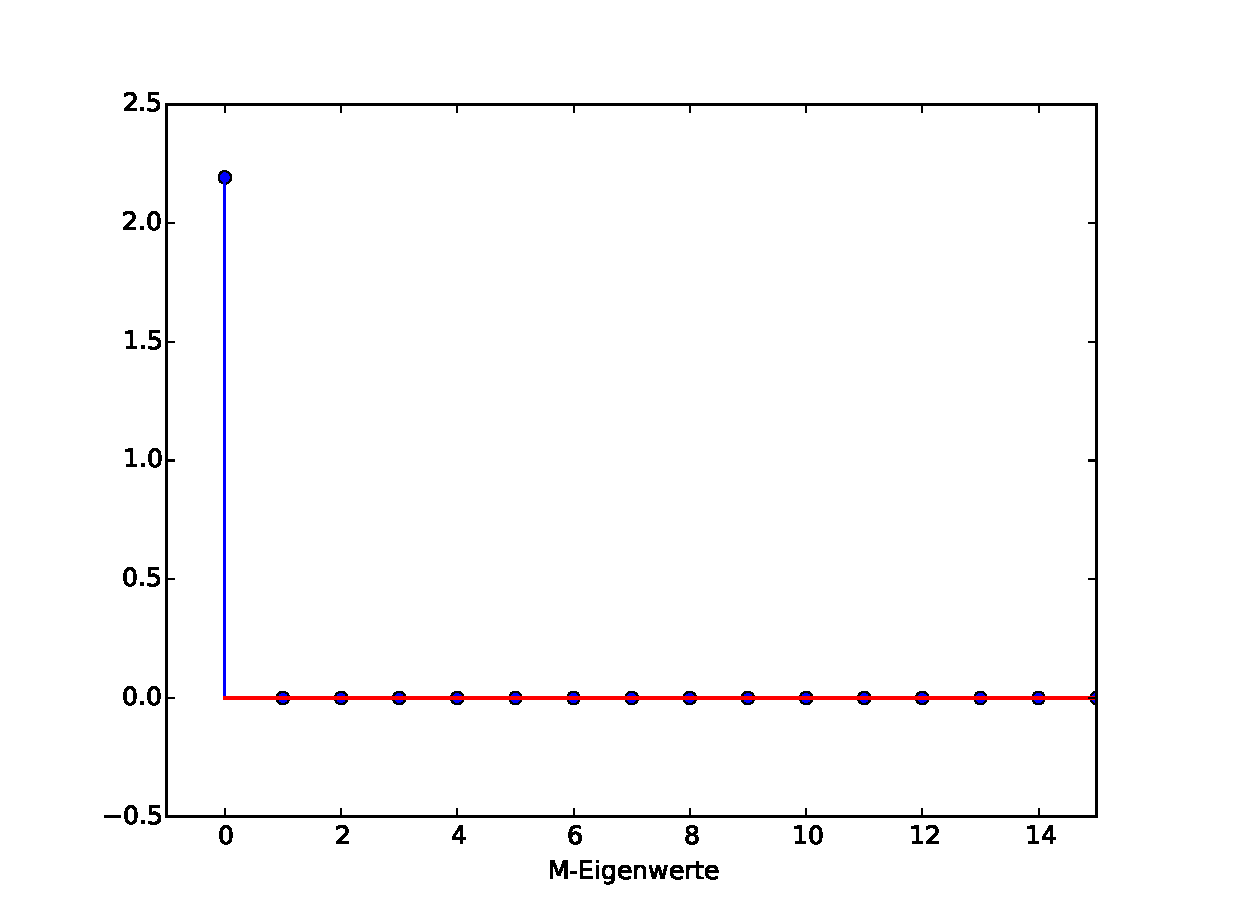
\includegraphics[scale=0.5]{images/OneDominant}
	\caption{Eigenwerte eines mit $M = 16$ Subträgern abgetasteten Zweipfadkanals}
	\label{fig:OneDominant}

\end{figure}

In Abbildung \ref{fig:OneDominant} sind die Eigenwerte eines Zweipfadkanals, welcher mit 16 Subträgern abgetastet wurde, dargestellt. Man erkennt, dass nur ein dominanter Eigenwert vorhanden ist und die restlichen Eigenwerte nahe der Null liegen, da \gls{symb:sigman} verhältnismäßig klein ist. 
Deshalb erfordert es einige Vorverarbeitungsmaßnahmen, um die Pfade unterscheiden zu können. Diese Techniken sind sogenannte \emph{Smoothing-Techniques} und werden im Folgenden genauer erläutert. 

\subsection{Smoothing-Techniques}
\label{chap3.3.1:Smoothing}
Mithilfe der Eigenwertzerlegung der Kanalschätzung, werden Signal- und Rauschraum getrennt. Das bedeutet, dass zwei Ebenen aufgespannt werden, die orthogonal aufeinander stehen. In der einen Ebene befinden sich alle Eigenvektoren, die zu den dominanten Eigenwerten gehören, in der Anderen die Restlichen. Die dominanten Eigenwerte werden dem Nutzsignal zugeordnet. Wenn die Signalanteile jedoch stark korreliert sind, gibt es nur einen dominanten Eigenwert und somit nur einen Eigenvektor. In Abbildung \ref{fig:SmoothingVektor} ist dieser Vektor schwarz gekennzeichnet. Dieser setzt sich aus den Vektoren des Mehrwegekanals zusammen, welche hellgrau dargestellt sind. Ein Vektor reicht jedoch nicht aus um die Ebene des Signalraums zu definieren. Die \emph{Smoothing}-Techniken versuchen diesen Summenvektor in zwei Anteile zu zerlegen. Es gibt zwei Methoden \emph{Smoothing} zu implementieren. Beide versuchen im wesentlichen diesen Summenvektor zu skalieren. Dies ist eine lineare Operation und erzeugt damit zwei Vektoren, in grün und rot, welche Linearkombinationen aus den Anteilen des ursprünglichen Vektors sind. 

\begin{figure}[htbp]
	\centering
	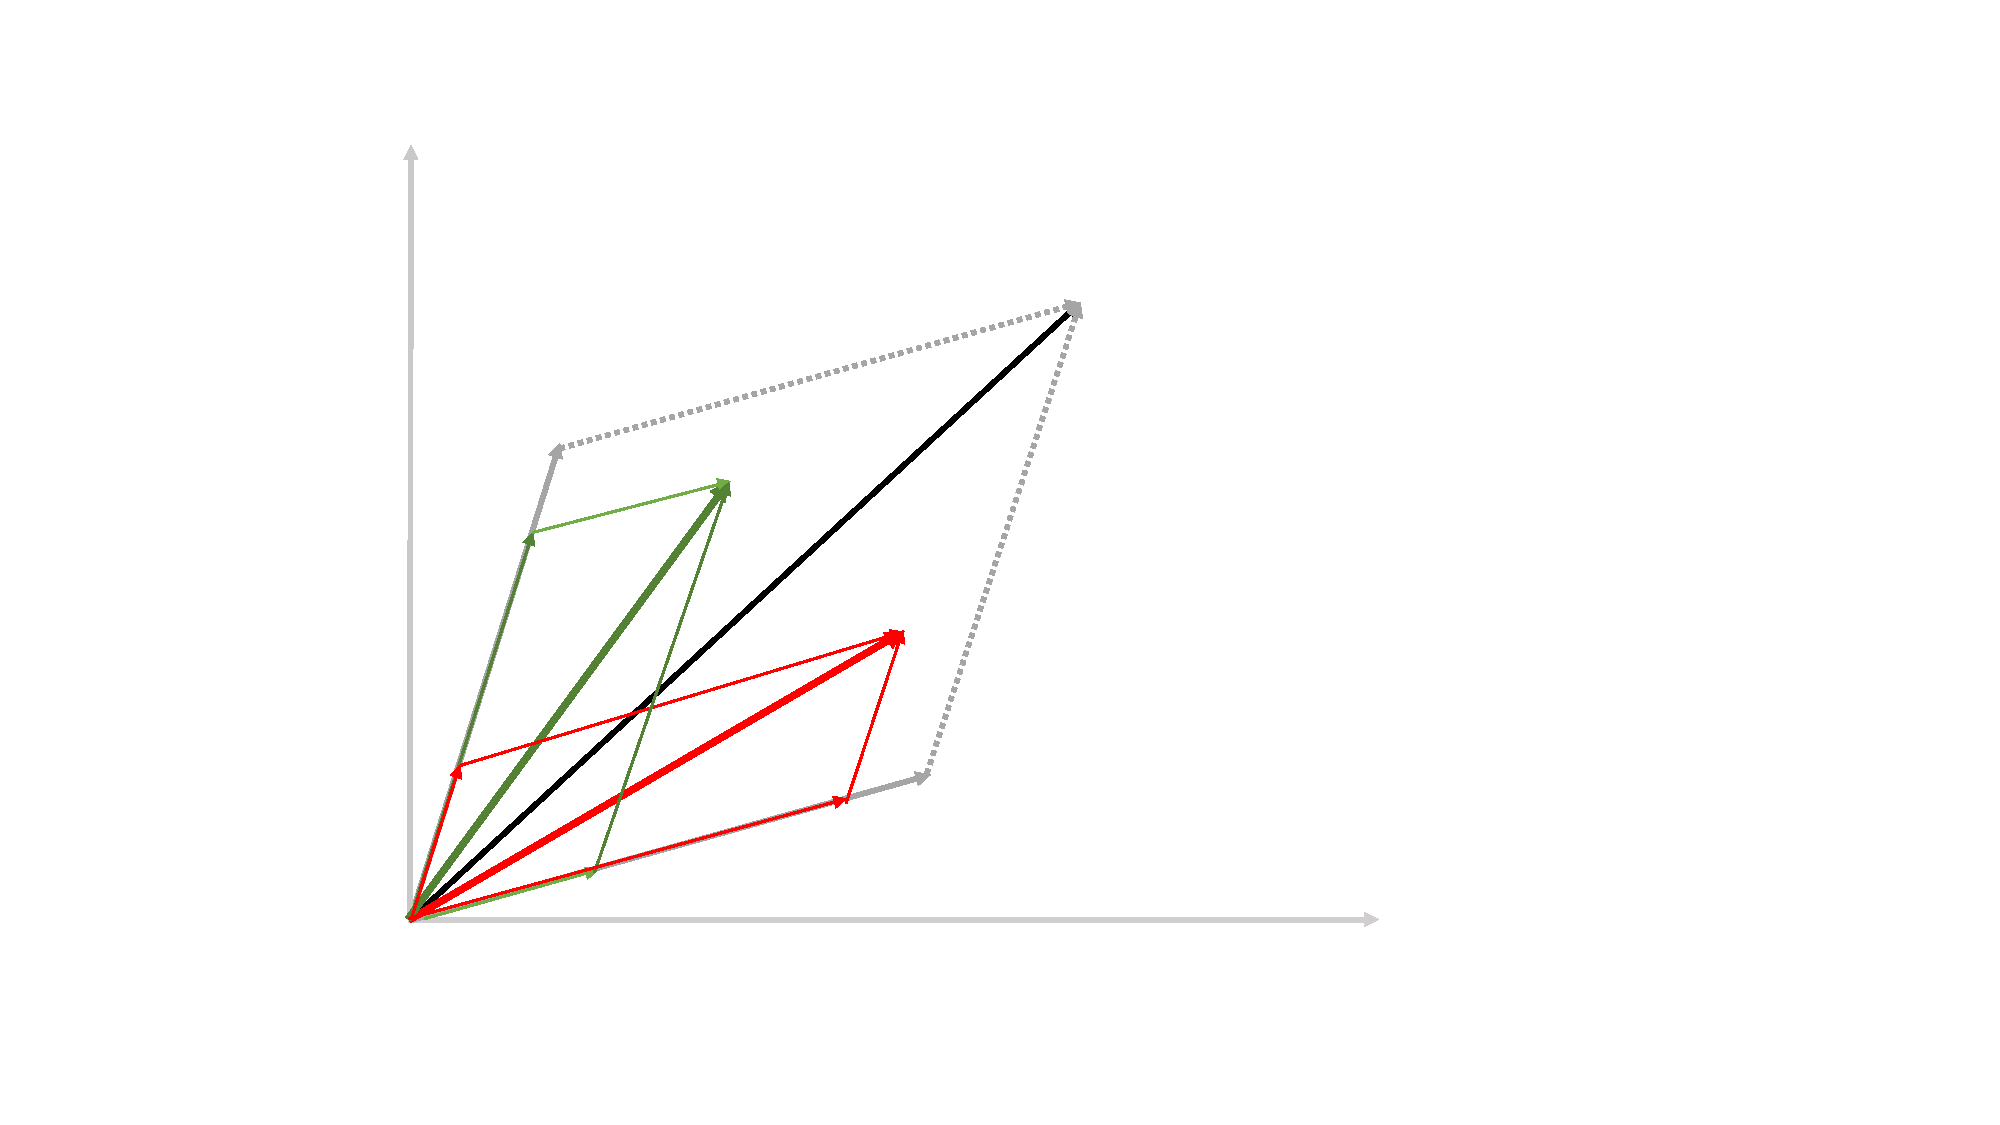
\includegraphics[scale=0.5]{images/SmoothingVektoren}
	\caption{Ergebnis des Smoothings in der Ebene des Signalraums}
	\label{fig:SmoothingVektor}
\end{figure}

Wie man in der Abbildung erkennen kann, ändert das Smoothing nichts an der Phase der Vektoren der zwei Pfade. 

Eine Methode, Smoothing zu implementieren, ist es, die Phasenrampe zu transponieren und zu spiegeln, sodass eine weitere identische Phasenrampe entsteht. Diese beiden Rampen haben, durch die vorher genannten Operationen, unterschiedliche Vorfaktoren. Dies führt zur gewünschten Skalierung. 


Eine weitere Möglichkeit ist es, die Phasenrampe in zwei Abschnitte zu unterteilen. Da der erste Wert von $\mathbf{v}(\tau) = [1, e^{-j\omega}, \ldots, e^{-j(M-1)\omega}]^T$, 1 ist und der zweite eine Exponentialfunktion, kann der zweite Abschnitt der Phasenrampe als $e^{-j\omega}$ multipliziert mit dem ersten darstellen werden. Damit wurde wieder durch unterschiedliche Vorfaktoren eine Skalierung bewerkstelligt.
In \cite{smoothing} wird gezeigt, dass, um $L$ Signale auflösen zu können, $M > L$ Phasenabschnitte benötigt werden. 
In Abbildung \ref{fig:DominantE} wurde letzteres Smoothing-Verfahren beispielhaft angewendet. Es wird ersichtlich, dass im Vergleich zu Abbildung \ref{fig:OneDominant} nun zwei Eigenwerte deutlich über dem Rauschniveau liegen. Bei Betrachtung der Anzahl der Eigenwerte, kann festgestellt werden, dass sie nicht der Anzahl M entspricht. Dieses Smoothingverfahren opfert eine Dimension des Rauschraums, um die zusätzliche Dimension im  Signalraum auflösen zu können.

\begin{figure}[htbp]
	\centering
	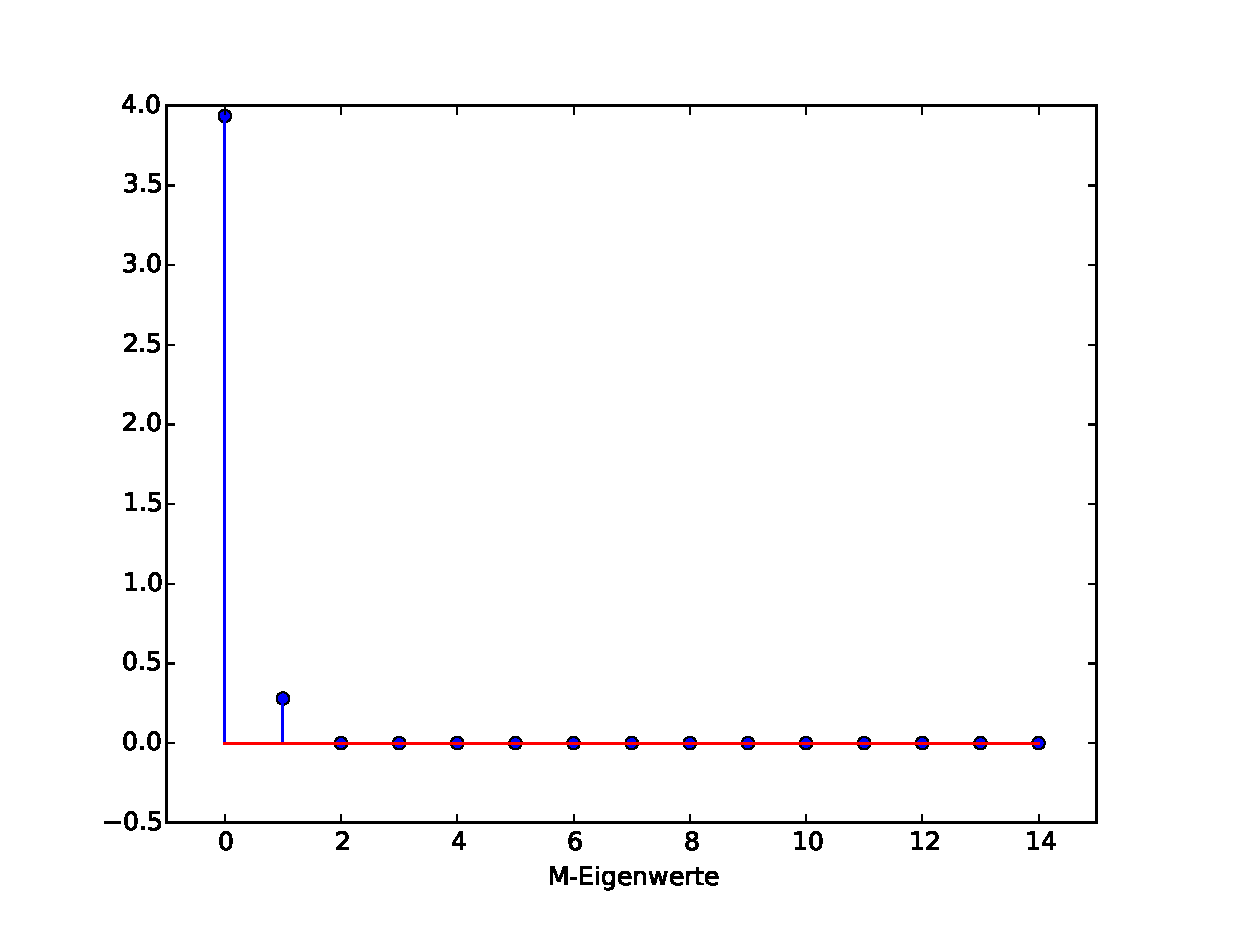
\includegraphics[scale=0.5]{images/DominantE}
	\caption{Eigenwerte eines mit M = 16 Subträgern abgetasteten Zweipfadkanal}
	\label{fig:DominantE}
\end{figure}

Nachdem die Korrelationsmatrix durch Smoothing Algorithmen modifiziert wurde, können die Subraumalgorithmen angewendet werden, um die Signale zu identifizieren. Diese werden ausführlich in \cite{kammeyer} erklärt. 

\subsection{MUSIC (MUltiple SIgnal Classification)}
\label{chap3.3.2:MUSIC}
Der MUSIC (MUltiple SIgnal Classification) Algorithmus zerlegt die Korrelationsmatrix der Kanalschätzung in ihre Eigenwerte. Da $\mathbf{VA_{aa}V^H}$ eine hermitesche Matrix ist, kann sie mittels Eigenwerten und Eigenvektoren diagonalisiert werden. 

\begin{equation}
	\label{eq:Eigenwertzerlegung}
	\mathbf{VA_{aa}V^H} = \mathbf{U} \Sigma \mathbf{U^{-1}}
\end{equation} 

$\Sigma = diag(\lambda_1, \ldots, \lambda_L, 0, \ldots, 0)$ ist die Diagonalmatrix der Eigenwerte und \\
$\mathbf{U}=[\mathbf{u_1, \ldots, u_L,u_{L+1},\ldots, u_M}] = [\mathbf{U_s}|\mathbf{U_n}]$ die Matrix der Eigenvektoren, aufgeteilt in Signal- und Rauschanteil. Die $L$ Eigenvektoren des Signalraums sind zu den Restlichen orthogonal. Somit sind die $M - L$ letzten Vektoren eine Basis für den Rauschraum. Daher muss für die gesuchten Vektoren $\mathbf{v}(\tau)$ gelten:

\begin{equation}
	\label{music bedingung}
	\mathbf{U_n^H}\cdot \mathbf{v}(\tau) = 0
\end{equation}

Um die zu den Signalen zugehörigen $\tau$ zu finden, wird das MUSIC-Spektrum(\ref{Music-Spektrum}) gebildet und dessen Maxima gesucht. 

\begin{equation}
	\label{Music-Spektrum}
	S(\tau) = \frac{1}{||\mathbf{U_n^H}\cdot \mathbf{v}(\tau)||^2}
\end{equation}

Das Suchen der Maxima in einem solchen MUSIC-Spektrum, ist mit hohem Rechenaufwand verbunden. Deshalb wird bei der Implementierung das Root-Music-Verfahren angewendet. Bei diesem  Verfahren werden mithilfe der Vektoren $v(z)$, direkt Nullstellen von $||\mathbf{U_n} \cdot \mathbf{v(z)}||^2$ in der z-Ebene berechnet.
In dieser Ebene ist das System, welches das Empfangssignal erzeugt hat, mit Pol- und Nullstellen um den Einheitskreis beschrieben. 

\subsection{ESPRIT (Estimation of Signal Paramters via Rotational Invariance Techniques)}
\label{chap3.3.3:ESPRIT}
ESPRIT ist ein weiteres Verfahren, das eine Eigenwertzerlegung der Kanalschätzung vornimmt. Es ist, wie der Root-MUSIC Algorithmus, wesentlich rechenärmer als das konventionelle MUSIC Verfahren. Das Verfahren teilt die, mit $M$-Samples abgetastete, Übertragungsfunktion $\mathbf{h}$ in zwei Frequenzbereiche auf. Dadurch ergeben sich zwei neue Matrizen $\mathbf{V_1} = \mathbf{|0]V}$ und $\mathbf{V_2} = \mathbf{[0|I]V}$, die für jeden Umwegpfad $L$ um dessen Laufzeit zueinander verdreht sind. Dieser Zusammenhang kann mit einer weiteren Matrix wie folgt ausgedrückt werden: 

\begin{equation}
	\label{eq:Drehmatrix}
	\mathbf{V_1} = \mathbf{\Omega V_2}  \;\;\;  mit \;\;\; \mathbf{\Omega} = diag(e^{j\omega_1}, \ldots, e^{j\omega_L} )
\end{equation} 

Die Eigenwerte $\nu_l$ der Matrix $\mathbf{\Omega}$ führen zu den gesuchten Verzögerungen $\tau_l$.
Da die gesuchten Vektoren $v(\tau)$ im Signalraum liegen, existiert eine invertierbare Transformationsmatrix, die den Zusammenhang \eqref{eq:Signalraum und V} herstellt.  

\begin{equation}
	\label{eq:Signalraum und V}
	\mathbf{U_s} = \mathbf{VT}
\end{equation}

Mit diesem Zusammenhang kann die Gleichung \eqref{eq:Drehmatrix} überführt werden in:

\begin{equation}
	\label{eq:berechnung von Psi}
	\mathbf{[0|1]U_s} = \mathbf{V_2T} = \mathbf{V_1\Omega T} = \mathbf{V_1T} \;\;\mathbf{T^{-1}\Omega T} = \mathbf{[0|1]U_s \Psi}
\end{equation}

Weil $\mathbf{\Psi}$ und $\mathbf{\Omega}$ ähnliche Matrizen sind, haben sie die selben Eigenwerte. 
Nun kann aus der Korrelationsmatrix die Matrix $\mathbf{\Psi}$ und daraus die Laufzeiten aller Pfade bestimmt werden. Die Gleichung \eqref{eq:berechnung von Psi} stellt dabei ein \emph{total-least-squares-Problem} dar. 
Das bedeutet, dass eine Matrix $\mathbf{\Psi}$ gefunden werden muss, die den kleinsten quadratischen Fehler beim erfüllen dieser Gleichung macht.
Die Lösung eines solchen Gleichungssystems kann mittels Singulärwertzerlegung und \emph{least-squares}-Ansatz gefunden werden.
Der ESPRIT-Algorithmus entspricht demnach einer Phasendifferenzschätzung mit Mehrwege-Auflösungsvermögen, da die Matrix $\mathbf{\Psi}$ die Phasenverdrehung zweier Frequenzabschnitte repräsentiert. 


